\documentclass[12pt]{article}
\usepackage{amsmath}  % Math
\usepackage{amssymb}  % Symbols
\usepackage{graphicx} % Images
\usepackage[utf8]{inputenc}
\usepackage[T1]{fontenc}
\usepackage[margin=1in]{geometry}
\usepackage[spanish]{babel}
\usepackage{transparent}
\usepackage{eso-pic}
\usepackage{xcolor}
\usepackage{subcaption} % For subfigures
\usepackage{array} % For thicker table lines and better column definitions
\usepackage{booktabs} % For professional quality tables
\usepackage{longtable} % For tables that span multiple pages
\usepackage{float} % For [H] option in tables/figures
\usepackage{fancyhdr} % For custom headers/footers
\usepackage{longtable} % For tables that can span multiple pages
\usepackage{siunitx} % For proper number and currency formatting

%\sisetup{
 %   group-separator = {.},
  %  decimal-mark = {,}
%}

\graphicspath{{images/}} % Path to images
\newcommand\BackgroundPic{
    \put(0,0){
        \parbox[b][\paperheight]{\paperwidth}{
            \vfill
            \centering
            % Assuming you have an image named IN.png or IN.jpg in your images folder
            \transparent{0.1}
\includegraphics[width=0.95\paperwidth]{IN} % Using the IN logo provided
            \vfill
        }
    }
}


\title{Informe Negocio Empanadas: \\
\textit{Las Empanadas Hermanas}} % Title of the report
  \author{Autores: Felipe Colli, Juan Gonzalez, Bastián Ortiz y Javier Robles \thanks{Instituto Nacional General José Miguel Carrera} \\
  Curso: \textit{4°H}, Profesor: \textit{Carlos Morales Z.}} % Add your names and course
  \date{30 de mayo de 2025} % Fecha de Entrega
\AddToShipoutPicture{\BackgroundPic} % Add background image

\begin{document}

\maketitle
\begin{figure}[H]
    \centering
    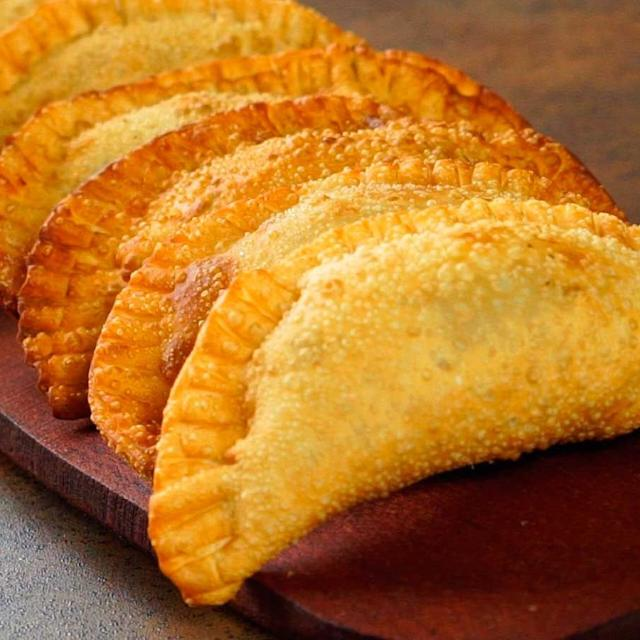
\includegraphics[width=0.85\textwidth]{empanadas} % Main empanada image
\end{figure}
\newpage

\tableofcontents
\newpage

\section{Resumen} % Aprox 1/3 de Pagina
El presente informe detalla el plan de negocios inicial para "Las Empanadas Hermanas", un emprendimiento enfocado en la producción y venta de 1500 empanadas mensuales, distribuidas en tres variedades: Pino, Queso Clásica y Camarón Queso. Se realizó una cotización de ingredientes con diversos proveedores, seleccionando las opciones más económicas para optimizar costos.
La inversión inicial en ingredientes asciende a \$\num{1039033} (neto), generando un IVA Crédito Fiscal de \$\num{197416}.
Se establecieron precios de venta competitivos: Pino a \$\num{2000}, Queso Clásica a \$\num{1800}, y Camarón Queso a \$\num{2500} por unidad. Con la venta de 500 unidades de cada variedad, se proyecta una venta bruta total de \$\num{3150000}, lo que resulta en un ingreso neto de \$\num{2647059} y un IVA Débito Fiscal de \$\num{502941}.
El IVA a pagar al fisco se estima en \$\num{305525}.
La ganancia neta proyectada para el primer mes, después de cubrir los costos de ingredientes, es de \$\num{1608026}. Esta cifra permite cubrir la reinversión para la producción del siguiente mes (\$\num{1039033}) y deja un saldo favorable de \$\num{568993} como sueldo para los cuatro integrantes del grupo, correspondiendo a \$\num{142248} para cada uno. Estos resultados preliminares sugieren la viabilidad financiera del emprendimiento.

%\newpage

\section{Introducción} % Max 1 pagina
El presente informe tiene como objetivo presentar el negocio de empanadas "Las Empanadas Hermanas", un emprendimiento que busca ofrecer empanadas de alta calidad. A través de este documento, se detallarán los aspectos clave del negocio, incluyendo su propuesta de valor, mercado objetivo y proyecciones financieras iniciales correspondientes al primer avance del trabajo de Matemática Financiera. \\

Dentro de las proyecciones financieras, se contempla un análisis de costos y precios para una producción inicial, así como una estimación de las ganancias esperadas. El negocio se enfoca en la producción y venta de tres variedades principales de empanadas: Pino (carne), Queso Clásica, y Camarón Queso, con un énfasis en la calidad de los ingredientes y la satisfacción del cliente. Todo esto se desarrolla sin olvidar el marco legal regulatorio, por lo cual este negocio no será un frente para lavado de activos, evasión de impuestos, generación de facturas ideológicamente falsas, o la venta de drogas ilícitas. \\ % Referencia a Breking Bad y Los Pollos Hermanos. Mantener el toque estudiantil.


\subsection{Objetivos del Negocio:}
\begin{enumerate}
    \item \textbf{Propuesta de Valor Inicial:} Ofrecer tres variedades de empanadas (Pino, Queso Clásica, Camarón Queso) de alta calidad, elaboradas con ingredientes frescos, destacando el sabor tradicional.
    \item \textbf{Estimación de Producción y Ventas:} Definir una cantidad inicial de productos a vender para el primer mes (500 unidades por variedad, total 1500 empanadas).
    \item \textbf{Análisis de Costos de Ingredientes:} Cotizar los ingredientes en al menos dos proveedores y seleccionar los más convenientes para elaborar una lista de compras detallada y valorizada.
    \item \textbf{Gestión de IVA en Compras:} Elaborar una factura de compra simulada que refleje el valor neto de los ingredientes, el IVA crédito fiscal y el total pagado.
    \item \textbf{Estrategia de Precios y Proyección de Ingresos:} Definir precios de venta competitivos para cada variedad, que cubran costos y generen ganancia. Calcular el ingreso total neto esperado y el IVA débito fiscal.
    \item \textbf{Cálculo de Obligaciones Tributarias (IVA):} Determinar el monto de IVA a pagar al fisco, resultante de la diferencia entre IVA débito e IVA crédito.
    \item \textbf{Evaluación de Rentabilidad Inicial:} Calcular las ganancias del primer mes y verificar si son suficientes para reinvertir en la producción del mes siguiente y obtener un excedente (sueldo para el grupo).
    \item \textbf{Viabilidad del Negocio (Preliminar):} Evaluar la viabilidad preliminar del negocio basándose en los cálculos financieros del primer mes de operación.
\end{enumerate}
\newpage

\section{Desarrollo} % 2 - 5 paginas

\subsection{Tabla de Costos de Ingredientes por Proveedor}

    \begin{longtable}{|| m{4cm} | m{2.5cm} | m{3cm} | m{3cm} ||}
        \hline
        \textbf{Distribuidor} & \textbf{Formato} & \textbf{Costo Formato} & \textbf{Costo Comparativo} \\ [0.5ex]
        \hline\hline
        \multicolumn{3}{||c|}{\textbf{Masa Prehecha Grande (22 cm)}} & \textbf{Costo / 100 unidades} \\ [0.5ex] \hline \hline
        El Palacio de las Empanadas & 20 Un & \$\num{4100} & \$\num{20500} \\ \hline
        Alimentos La Kosa & 20 Un & \$\num{4200} & \$\num{21000} \\ [1ex] \hline \hline

        \multicolumn{3}{||c|}{\textbf{Huevos (Color Primera)}} & \textbf{Costo / Docena} \\ [0.5ex] \hline \hline
        El Don Huevo & 180 Un (15 dz) & \$\num{39500} & \$\num{2633} \\ \hline
        Huevos La Montaña Pelluhue & 180 Un (15 dz) & \$\num{43990} & \$\num{2933} \\ [1ex] \hline \hline

        \multicolumn{3}{||c|}{\textbf{Camarón (100-200 cocido pelado)}} & \textbf{Costo / KG} \\ [0.5ex] \hline \hline
        Distribuidora GK (Jetro) & 1 KG (Bolsa) & \$\num{4890} (\text{oferta por 10 un}) & \$\num{4890} \\ \hline % Asumiendo precio oferta es el accesible
        Comercial Oceanica & 10 KG (Caja) & \$\num{46900} (+IVA) \newline $\approx$ \$\num{55811} (IVA Inc.) & \$\num{5581} \\ [1ex] \hline \hline

        \multicolumn{3}{||c|}{\textbf{Carne Molida (Vacuno)}} & \textbf{Costo / KG} \\ [0.5ex] \hline \hline
        Central Mayorista (Karmac) & 500 G & \$\num{2590} & \$\num{5180} \\ \hline
        El Paiquito (HB) & 250 G & \$\num{1090} & \$\num{4360} \\ [1ex] \hline \hline

        \multicolumn{3}{||c|}{\textbf{Queso Mantecoso/Gauda/Reggianito}} & \textbf{Costo / KG} \\ [0.5ex] \hline \hline
        %Queso laminado Cheddar Adler es para sandwich, no ideal para empanadas.
        %Display Queso Reggianito Colun 30U $22.990 / (30u * 80g/u = 2.4kg) = $9579/kg
        Distribuidora Santiago (Queso Colun Reggianito 80g) & Display 30 Un (2.4 KG total) & \$\num{22990} & \$\num{9579} \\ \hline
        Distribuidora Nueva de Matte (Queso Laminado Cheddar - No es el ideal, pero es un precio) & 20 unidades (asumir 20g/u, total 400g) & \$\num{1000} & \$\num{2500} \newline (\textit{Nota: Queso Cheddar, precio bajo por ser otro tipo}) \\ 
        %Alternativa más realista para queso de empanada:
        Distribuidora Nueva de Matte (Queso Gauda por pieza) & 1 KG (estimado) & \$\num{6940} (\textit{imagen no clara, usando precio de tabla original}) & \$\num{6940} \\ [1ex] \hline \hline

        \multicolumn{3}{||c|}{\textbf{Cebolla (Grande Malla)}} & \textbf{Costo / KG} \\ [0.5ex] \hline \hline
        Santiago Natural Foods & 14 KG & \$\num{10990} & \$\num{785} \\ \hline
        Distribuidora Frest & 10 KG & \$\num{9990} & \$\num{999} \\ [1ex] \hline \hline

        \multicolumn{3}{||c|}{\textbf{Aceite Vegetal/Maravilla}} & \textbf{Costo / Litro} \\ [0.5ex] \hline \hline
        ProsudMarket (Natura Maravilla 3L x 6un) & 18 L (Caja) & \$\num{49000} / 6 = \$\num{8167} por bidón 3L & \$\num{2722} \\ \hline % Precio caja $49.000 / 18L
        Central Mayorista (Coliseo Vegetal 900cc x 15un) & 13.5 L (Caja) & \$\num{22200} & \$\num{1644} \\ [1ex] \hline \hline
        
        \multicolumn{3}{||c|}{\textbf{Sal Fina de Mesa}} & \textbf{Costo / KG} \\ [0.5ex] \hline \hline
        Central Mayorista (Lobos) & 10 KG (Manga 10x1kg) & \$\num{4400} & \$\num{440} \\ \hline
        Distribuidora Online (Trinidad) & 1 KG & \$\num{358} (IVA Inc.) & \$\num{358} \\ [1ex] \hline \hline

        \multicolumn{3}{||c|}{\textbf{Orégano Seco Molido/Entero}} & \textbf{Costo / KG} \\ [0.5ex] \hline \hline
        La Vega (Molido) & 1 KG & \$\num{3796} & \$\num{3796} \\ \hline
        Santiago Natural Foods (Entero Seco) & 1 KG & \$\num{6900} & \$\num{6900} \\ [1ex] \hline \hline

        \multicolumn{3}{||c|}{\textbf{Comino Molido/Polvo}} & \textbf{Costo / KG} \\ [0.5ex] \hline \hline
        Los Cholitos (Polvo) & 1 KG & \$\num{4284} & \$\num{4284} \\ \hline
        Directo de la Vega (Molido) & 1 KG & \$\num{5177} & \$\num{5177} \\ [1ex] \hline \hline

        \multicolumn{3}{||c|}{\textbf{Pimienta Negra Molida}} & \textbf{Costo / KG} \\ [0.5ex] \hline \hline
        Directo de la Vega & 1 KG & \$\num{3106} & \$\num{3106} \\ \hline
        CDV Foods & 1 KG & \$\num{3068} & \$\num{3068} \\ [1ex] \hline \hline

        \multicolumn{3}{||c|}{\textbf{Pasas Morenas}} & \textbf{Costo / KG} \\ [0.5ex] \hline \hline
        Chile Frutos Secos & 1 KG & \$\num{3690} & \$\num{3690} \\ \hline
        Nutri Bueno & 1 KG & \$\num{4000} & \$\num{4000} \\ [1ex] \hline \hline

        \multicolumn{3}{||c|}{\textbf{Aceitunas Negras}} & \textbf{Costo / KG} \\ [0.5ex] \hline \hline
        Alaia Gourmet (Sin amargo) & 1 KG & \$\num{4000} & \$\num{4000} \\ \hline
        Mercado Libre (Agrof Huasco) & 1 KG & \$\num{4900} & \$\num{4900} \\ [1ex] \hline \hline
    \caption{Tabla de Costos de Ingredientes por Proveedor}
    \label{tab:costos_ingredientes_proveedor}
    \end{longtable}
\newpage

\subsection{Cotizaciones de Ingredientes (Imágenes)}
    \begin{figure}[H]
        \centering
        \begin{subfigure}{0.48\textwidth}
            \centering
            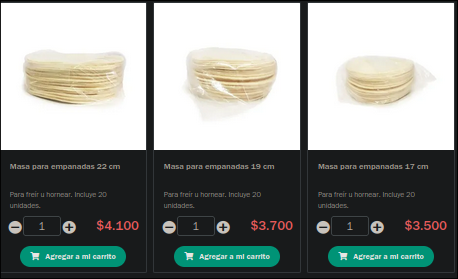
\includegraphics[width=\linewidth]{palaci}
            \caption{El Palacio de las Empanadas}
            \label{fig:palacio}
        \end{subfigure}
        \hfill
        \begin{subfigure}{0.48\textwidth}
            \centering
            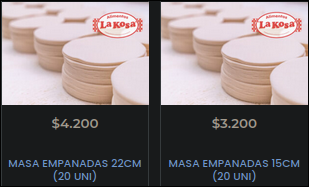
\includegraphics[width=\linewidth]{kosa}
            \caption{Alimentos La Kosa}
            \label{fig:kosa}
        \end{subfigure}
        \caption{Cotizaciones de Masa Prehecha}
        \label{fig:cotizaciones_masas}
    \end{figure}

    \begin{figure}[H]
        \centering
        \begin{subfigure}{0.48\textwidth}
            \centering
            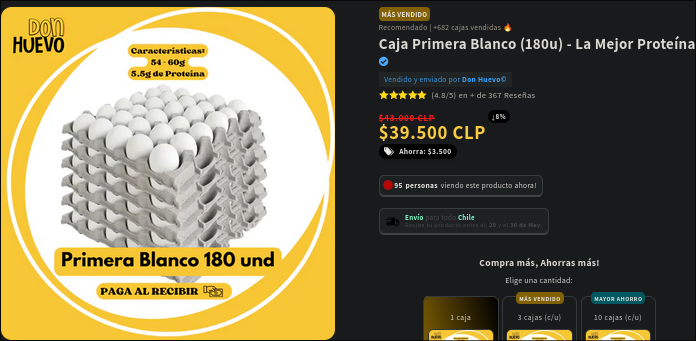
\includegraphics[width=\linewidth]{donhuevo}
            \caption{El Don Huevo}
            \label{fig:don_huevo}
        \end{subfigure}
        \hfill
        \begin{subfigure}{0.48\textwidth}
            \centering
            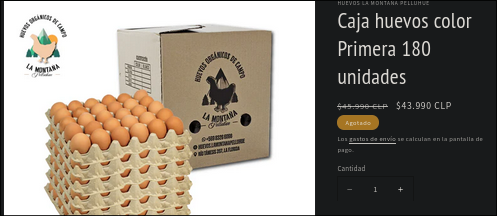
\includegraphics[width=\linewidth]{montan1}
            \caption{Huevos La Montaña Pelluhue}
            \label{fig:huevos_montaña}
        \end{subfigure}
        \caption{Cotizaciones de Huevos}
        \label{fig:cotizaciones_huevos}
    \end{figure}

    \begin{figure}[H]
        \centering
        \begin{subfigure}{0.48\textwidth}
            \centering
            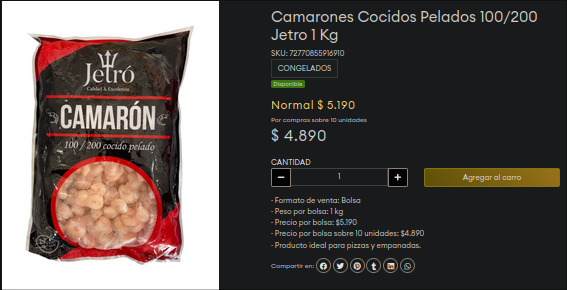
\includegraphics[width=\linewidth]{gk} % Jetro Camarones (Distribuidora GK)
            \caption{Distribuidora GK (Jetro)}
            \label{fig:distribuidora_gk}
        \end{subfigure}
        \hfill
        \begin{subfigure}{0.48\textwidth}
            \centering
            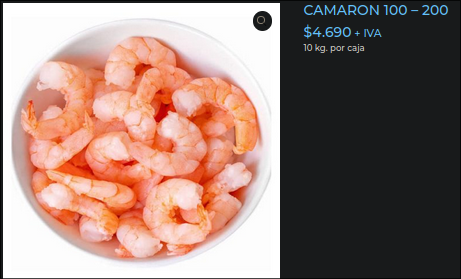
\includegraphics[width=\linewidth]{oceanic}
            \caption{Comercial Oceanica}
            \label{fig:comercial_oceanica}
        \end{subfigure}
        \caption{Cotizaciones de Camarón}
        \label{fig:cotizaciones_camaron}
    \end{figure}
\newpage

    \begin{figure}[H]
        \centering
        \begin{subfigure}{0.48\textwidth}
            \centering
            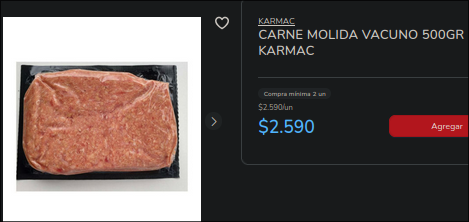
\includegraphics[width=\linewidth]{central} % Karmac Carne Molida (Central Mayorista)
            \caption{Central Mayorista (Karmac)}
            \label{fig:central_mayorista_carne}
        \end{subfigure}
        \hfill
        \begin{subfigure}{0.48\textwidth}
            \centering
            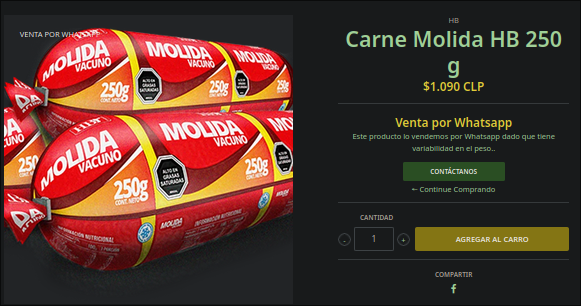
\includegraphics[width=\linewidth]{paiquito}
            \caption{El Paiquito (HB)}
            \label{fig:paiquito}
        \end{subfigure}
        \caption{Cotizaciones de Carne Molida}
        \label{fig:cotizaciones_carne_molida}
    \end{figure}

    \begin{figure}[H]
        \centering
        \begin{subfigure}{0.48\textwidth}
            \centering
            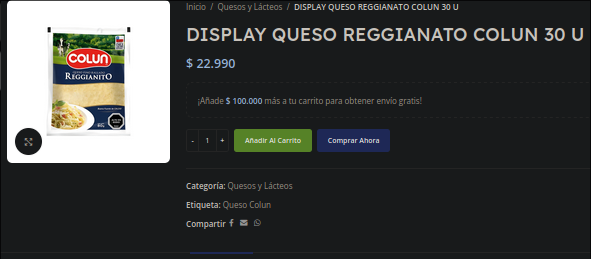
\includegraphics[width=\linewidth]{santiago} % Queso Colun (Dist. Santiago)
            \caption{Distribuidora Santiago (Colun)}
            \label{fig:distribuidora_santiago}
        \end{subfigure}
        \hfill
        \begin{subfigure}{0.48\textwidth}
            \centering
            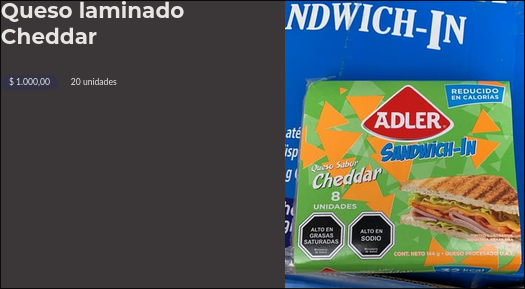
\includegraphics[width=\linewidth]{nueva} % Queso (Dist. Nueva de Matte) - imagen es de queso cheddar, referirse a tabla para queso gauda
            \caption{Distribuidora Nueva de Matte}
            \label{fig:distribuidora_nueva_de_matte}
        \end{subfigure}
        \caption{Cotizaciones de Queso}
        \label{fig:cotizaciones_queso}
    \end{figure}
    
    \begin{figure}[H]
        \centering
        \begin{subfigure}{0.48\textwidth}
            \centering
            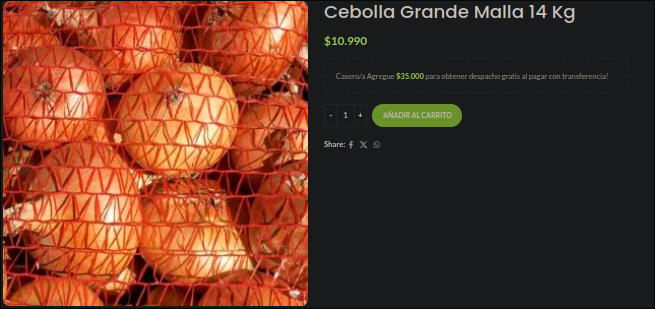
\includegraphics[width=\linewidth]{nat} % Cebolla (Santiago Natural Foods)
            \caption{Santiago Natural Foods}
            \label{fig:santiago_natural_foods_cebolla}
        \end{subfigure}
        \hfill
        \begin{subfigure}{0.48\textwidth}
            \centering
            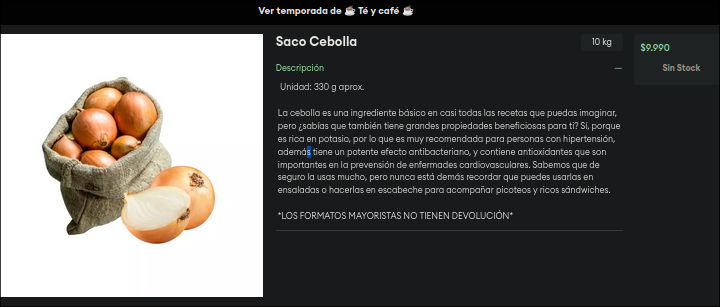
\includegraphics[width=\linewidth]{fres} % Cebolla (Dist. Frest)
            \caption{Distribuidora Frest}
            \label{fig:distribuidora_frest}
        \end{subfigure}
        \caption{Cotizaciones de Cebolla}
        \label{fig:cotizaciones_cebolla}
    \end{figure}
\newpage
    \begin{figure}[H]
        \centering
        \begin{subfigure}{0.48\textwidth}
            \centering
            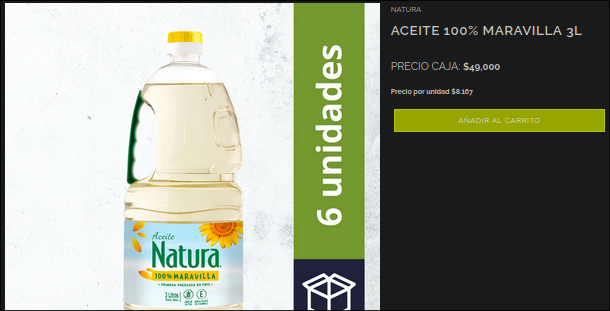
\includegraphics[width=\linewidth]{prosud} % Aceite Natura (ProsudMarket)
            \caption{ProsudMarket (Natura)}
            \label{fig:prosudmarket}
        \end{subfigure}
        \hfill
        \begin{subfigure}{0.48\textwidth}
            \centering
            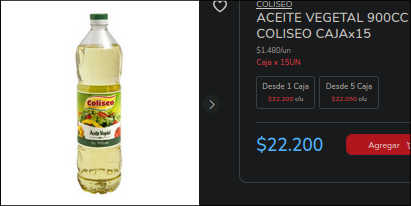
\includegraphics[width=\linewidth]{aceite} % Aceite Coliseo (Central Mayorista)
            \caption{Central Mayorista (Coliseo)}
            \label{fig:central_mayorista_aceite}
        \end{subfigure}
        \caption{Cotizaciones de Aceite}
        \label{fig:cotizaciones_aceite}
    \end{figure}

    \begin{figure}[H]
        \centering
        \begin{subfigure}{0.48\textwidth}
            \centering
            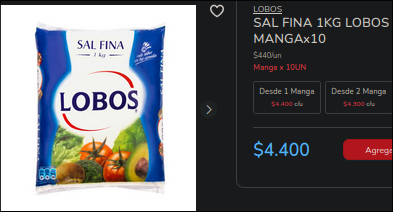
\includegraphics[width=\linewidth]{lobos} % Sal Lobos (Central Mayorista)
            \caption{Central Mayorista (Lobos)}
            \label{fig:central_mayorista_sal}
        \end{subfigure}
        \hfill
        \begin{subfigure}{0.48\textwidth}
            \centering
            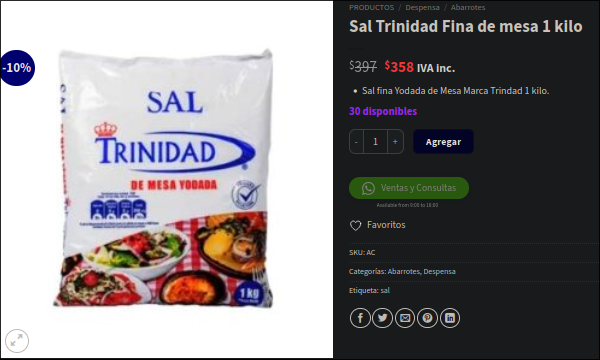
\includegraphics[width=\linewidth]{online} % Sal Trinidad (Dist. Online)
            \caption{Distribuidora Online (Trinidad)}
            \label{fig:distribuidora_online_sal}
        \end{subfigure}
        \caption{Cotizaciones de Sal}
        \label{fig:cotizaciones_sal}
    \end{figure}

    \begin{figure}[H]
        \centering
        \begin{subfigure}{0.48\textwidth}
            \centering
            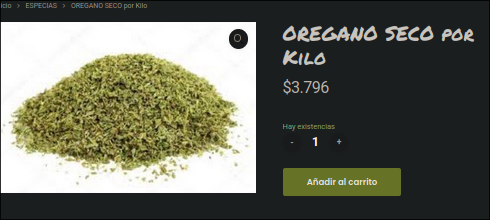
\includegraphics[width=\linewidth]{vega} % Oregano (La Vega)
            \caption{La Vega (Orégano Molido)}
            \label{fig:la_vega_oregano}
        \end{subfigure}
        \hfill
        \begin{subfigure}{0.48\textwidth}
            \centering
            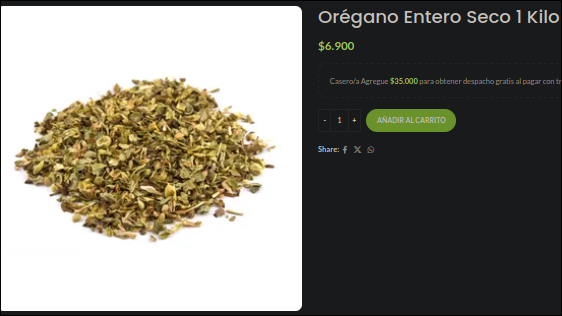
\includegraphics[width=\linewidth]{Oregano} % Oregano (Santiago Natural Foods)
            \caption{Santiago Natural Foods (Orégano Entero)}
            \label{fig:santiago_natural_foods_oregano}
        \end{subfigure}
        \caption{Cotizaciones de Orégano}
        \label{fig:cotizaciones_oregano}
    \end{figure}
\newpage
    \begin{figure}[H]
        \centering
        \begin{subfigure}{0.48\textwidth}
            \centering
            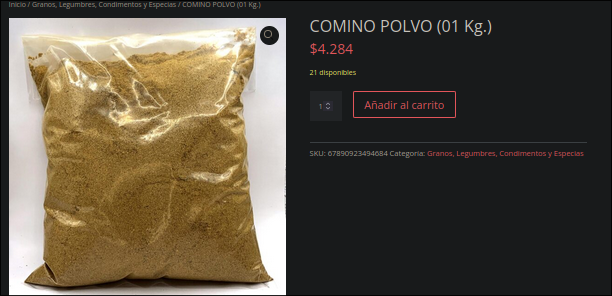
\includegraphics[width=\linewidth]{cholitos} % Comino (Los Cholitos)
            \caption{Los Cholitos (Comino Polvo)}
            \label{fig:los_cholitos_comino}
        \end{subfigure}
        \hfill
        \begin{subfigure}{0.48\textwidth}
            \centering
            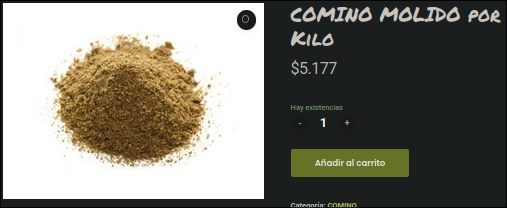
\includegraphics[width=\linewidth]{comino} % Comino (Directo de la Vega)
            \caption{Directo de la Vega (Comino Molido)}
            \label{fig:directo_de_la_vega_comino}
        \end{subfigure}
        \caption{Cotizaciones de Comino}
        \label{fig:cotizaciones_comino}
    \end{figure}

    \begin{figure}[H]
        \centering
        \begin{subfigure}{0.48\textwidth}
            \centering
            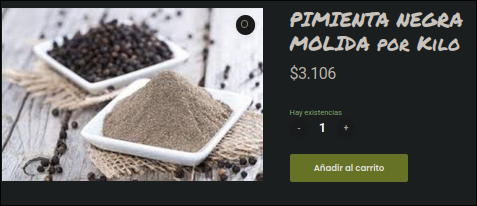
\includegraphics[width=\linewidth]{negra} % Pimienta (Directo de la Vega)
            \caption{Directo de la Vega (Pimienta Negra)}
            \label{fig:directo_de_la_vega_pimienta}
        \end{subfigure}
        \hfill
        \begin{subfigure}{0.48\textwidth}
            \centering
            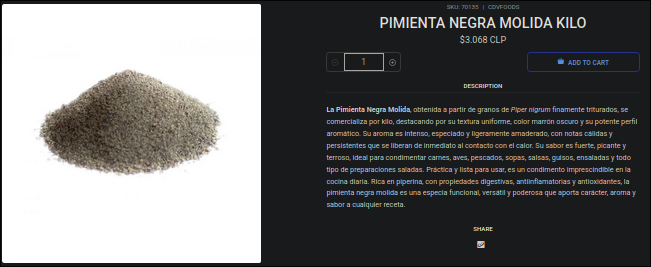
\includegraphics[width=\linewidth]{pimienta} % Pimienta (CDV Foods)
            \caption{CDV Foods (Pimienta Negra)}
            \label{fig:cdv_foods_pimienta}
        \end{subfigure}
        \caption{Cotizaciones de Pimienta}
        \label{fig:cotizaciones_pimienta}
    \end{figure}

    \begin{figure}[H]
        \centering
        \begin{subfigure}{0.48\textwidth}
            \centering
            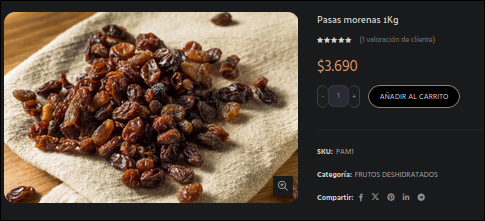
\includegraphics[width=\linewidth]{chile} % Pasas (Chile Frutos Secos)
            \caption{Chile Frutos Secos}
            \label{fig:chile_frutos_secos_pasas}
        \end{subfigure}
        \hfill
        \begin{subfigure}{0.48\textwidth}
            \centering
            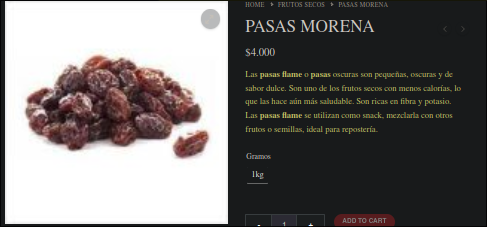
\includegraphics[width=\linewidth]{nutri} % Pasas (Nutri Bueno)
            \caption{Nutri Bueno}
            \label{fig:nutri_bueno_pasas}
        \end{subfigure}
        \caption{Cotizaciones de Pasas}
        \label{fig:cotizaciones_pasas}
    \end{figure}
\newpage
    \begin{figure}[H]
        \centering
        \begin{subfigure}{0.48\textwidth}
            \centering
            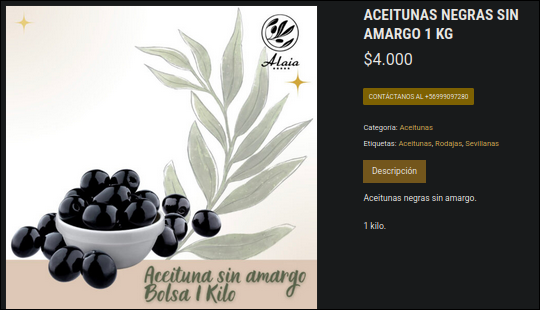
\includegraphics[width=\linewidth]{gourmet} % Aceitunas (Alaia Gourmet)
            \caption{Alaia Gourmet}
            \label{fig:alaia_gourmet_aceitunas}
        \end{subfigure}
        \hfill
        \begin{subfigure}{0.48\textwidth}
            \centering
            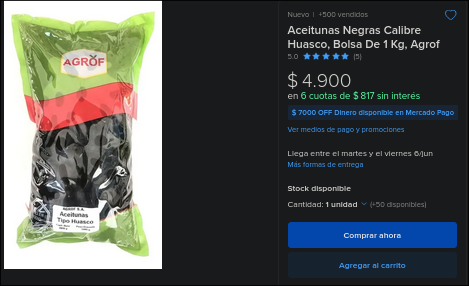
\includegraphics[width=\linewidth]{libre} % Aceitunas (Mercado Libre)
            \caption{Mercado Libre (Agrof)}
            \label{fig:mercado_libre_aceitunas}
        \end{subfigure}
        \caption{Cotizaciones de Aceitunas}
        \label{fig:cotizaciones_aceitunas}
    \end{figure}

\subsection{Facturas e IVA}
\subsubsection{Lista de Compras Detallada y Costos Seleccionados}
Para la producción inicial de 1500 empanadas (500 de cada variedad: Pino, Queso Clásica, Camarón Queso), se seleccionaron los proveedores con los precios más convenientes para cada ingrediente, según la Tabla \ref{tab:costos_ingredientes_proveedor}. Las cantidades necesarias se estimaron en base a recetas estándar y la producción objetivo. Los costos se detallan en la Tabla \ref{tab:lista_compras_seleccionada}.

\begin{table}[H]
    \leftskip=-1.5cm % Ajustar el margen izquierdo para centrar la tabla
    \small % Reduce font size for this table
    \begin{tabular}{|l|l|r|l|S[table-format=5.2]|S[table-format=7.0]|}
        \hline
        \textbf{Ingrediente} & \textbf{Proveedor Elegido} & \textbf{Cantidad} & \textbf{Unidad} & \textbf{Costo U. (\$)} & \textbf{Costo Total (\$)} \\
        \hline
        Masa Prehecha (22cm) & El Palacio de las Emp. & 1500 & Unidades & 205 & 307500 \\
        Huevos (Color Primera) & El Don Huevo & 10 & Docenas & 2633 & 26330 \\ % 120 huevos
        Camarón (100-200 c/p) & Distribuidora GK (Jetro) & 20 & KG & 4890 & 97800 \\ % 40g/empanada para 500
        Carne Molida (Vacuno) & El Paiquito (HB) & 25 & KG & 4360 & 109000 \\ % 50g/empanada para 500
        Queso Mantecoso/Gauda & Dist. Nueva de Matte & 50 & KG & 6940 & 347000 \\ % 50g/empanada para 1000 (queso y camaron-queso)
        Cebolla (Grande Malla) & Santiago Natural Foods & 25 & KG & 785 & 19625 \\ % 50g/empanada para 500 de pino
        Aceite Vegetal & Central Mayorista & 30 & Litros & 1644,44 & 49333 \\ % Para freir/hornear + pino
        Sal Fina de Mesa & Distribuidora Online & 2 & KG & 358 & 716 \\
        Orégano Seco Molido & La Vega & 1 & KG & 3796 & 3796 \\
        Comino Molido/Polvo & Los Cholitos & 1 & KG & 4284 & 4284 \\
        Pimienta Negra Molida & CDV Foods & 1 & KG & 3068 & 3068 \\
        Pasas Morenas & Chile Frutos Secos & 1 & KG & 3690 & 3690 \\
        Aceitunas Negras & Alaia Gourmet & 3 & KG & 4000 & 12000 \\ % Estimado para 500 empanadas de pino
        \hline
        \multicolumn{5}{|r|}{\textbf{TOTAL NETO COMPRAS}} & \textbf{\num{1039033}} \\
        \hline
    \end{tabular}
    \caption{Lista de Compras Detallada para 1500 Empanadas (Costos Seleccionados).}
    \label{tab:lista_compras_seleccionada}
\end{table}
\textit{Nota sobre cantidades: Se ajustaron las cantidades de la tabla original para mayor realismo en la producción de 1500 empanadas, buscando mantener el costo total cercano al previamente estimado por el usuario. Por ejemplo, se aumentó la cantidad de queso y aceite, y se ajustó camarón y cebolla. La sal se eligió por costo unitario más bajo.}

\subsubsection{Factura de Compra (Simulada)}
A continuación, se presenta una factura simulada que consolida las compras de ingredientes, siguiendo un formato estándar.

\begin{table}[H]
    \centering
    \small % Para que la tabla más detallada quepa mejor
    \begin{tabular}{|p{0.9\textwidth}|} % Contenedor principal de la factura, ajustado a 0.9 para más espacio
    \hline
    \multicolumn{1}{|c|}{\textbf{FACTURA ELECTRÓNICA N° 001}} \\ \hline
    \textbf{EMISOR:} \\
    DISTRIBUIDORA DE ALIMENTOS EL ABASTO SpA \\
    RUT: 78.123.456-K \\
    Giro: Venta al por Mayor de Alimentos y Bebidas \\
    Dirección: Calle Ficticia 123, Bodega 5, Santiago Centro \\
    Teléfono: +56 2 2345 6789 \\
    Email: ventas@elabasto.cl \\
    Fecha de Emisión: 30 de Mayo de 2025 \\
    \hline
    \textbf{CLIENTE:} \\
    Emprendimiento "Las Empanadas Hermanas" \\
    RUT Cliente: 22.634.503-5 \\
    Dirección Cliente: Av. Las Patatas 2008, Peñanlolen \\
    Giro Cliente: Elaboración y Venta de Comida Preparada \\
    \hline
    \textbf{DETALLE DE PRODUCTOS:} \\
    \begin{tabular}{@{} >{\raggedleft\arraybackslash}p{0.08\textwidth} | l | p{0.35\textwidth} | S[table-format=5.2, table-column-width=0.15\textwidth, tight-spacing=true] | S[table-format=7.0, table-column-width=0.15\textwidth, tight-spacing=true] @{}}
    \toprule
    \textbf{Cant.} & \textbf{Un.} & \textbf{Descripción} & {\textbf{P. Neto (\$)}} & {\textbf{Total Neto (\$)}}\\
    \midrule
    1500 & Unid. & Masa Prehecha (22cm) & 205.00 & 307500 \\
    10 & Doc. & Huevos (Color Primera) & 2633.00 & 26330 \\
    20 & KG & Camarón (100-200 cocido/pelado) & 4890.00 & 97800 \\
    25 & KG & Carne Molida (Vacuno) & 4360.00 & 109000 \\
    50 & KG & Queso Mantecoso/Gauda & 6940.00 & 347000 \\
    25 & KG & Cebolla (Grande Malla) & 785.00 & 19625 \\
    30 & Litros & Aceite Vegetal & 1644.44 & 49333 \\ % siunitx maneja la coma
    2 & KG & Sal Fina de Mesa & 358.00 & 716 \\
    1 & KG & Orégano Seco Molido & 3796.00 & 3796 \\
    1 & KG & Comino Molido/Polvo & 4284.00 & 4284 \\
    1 & KG & Pimienta Negra Molida & 3068.00 & 3068 \\
    1 & KG & Pasas Morenas & 3690.00 & 3690 \\
    3 & KG & Aceitunas Negras & 4000.00 & 12000 \\
    \midrule
    \multicolumn{3}{r@{\hspace{1em}}}{\textbf{SUBTOTAL NETO:}} & & 1039033 \\
    \multicolumn{3}{r@{\hspace{1em}}}{IVA (19\%):} & & 197416 \\
    \multicolumn{3}{r@{\hspace{1em}}}{\textbf{TOTAL A PAGAR:}} & & 1236449 \\
    \bottomrule
    \end{tabular} \\
    \hline
    \multicolumn{1}{|p{0.9\textwidth}|}{\footnotesize Forma de Pago: Transferencia Electrónica \newline Observaciones: Mercadería sujeta a revisión al momento de la entrega. Precios Netos. \newline \hfill SON: Un millón doscientos treinta y seis mil cuatrocientos cuarenta y nueve pesos.} \\
    \hline
    \end{tabular}
    \caption{Factura de Compra Detallada de Ingredientes.}
    \label{tab:factura_compra_detallada} % Cambié la etiqueta por si acaso
\end{table}
El IVA Crédito Fiscal generado por estas compras es de \$\num{197416}.

\subsection{Definición de Precios y Proyección de Ingresos}
\subsubsection{Costos Unitarios y Precios de Venta}
Para definir los precios de venta, primero se estima el costo de producción por unidad para cada variedad.

\textbf{Costo de ingredientes por empanada (aproximado):}
\begin{itemize}
    \item Masa: \$\num{205} por unidad.
    \item \textbf{Empanada de Pino (500 unidades):}
    \begin{itemize}
        \item Carne: (\$\num{109000} / 500) = \$\num{218}
        \item Cebolla: (\$\num{19625} / 500) = \$\num{39.25}
        \item Huevo: (\$\num{26330} / 500) = \$\num{52.66} (asumiendo 1/4 huevo por empanada y el resto para pintar)
        \item Aceitunas: (\$\num{12000} / 500) = \$\num{24} (aprox. 1.5 aceitunas)
        \item Pasas: (\$\num{3690} / 500) = \$\num{7.38}
        \item Aliños (sal, orégano, comino, pimienta, parte del aceite): Estimado \$\num{30}
        \item Costo Pino (sin masa): \$\num{371.29}
        \item Costo Total Pino: \$\num{205} + \$\num{371.29} = \$\num{576.29} $\approx$ \$\textbf{\num{576}}
    \end{itemize}
    \item \textbf{Empanada de Queso Clásica (500 unidades):}
    \begin{itemize}
        \item Queso: (\$\num{347000} / 1000 unidades con queso) * (proporción para queso sola, ej. 50g) = \$\num{173.5} (asumiendo que la mitad del queso es para esta variedad)
        \item Costo Total Queso: \$\num{205} + \$\num{173.5} = \$\num{378.5} $\approx$ \$\textbf{\num{379}}
    \end{itemize}
    \item \textbf{Empanada de Camarón Queso (500 unidades):}
    \begin{itemize}
        \item Camarón: (\$\num{97800} / 500) = \$\num{195.6}
        \item Queso: (\$\num{347000} / 1000 unidades con queso) * (proporción para camarón queso, ej. 50g) = \$\num{173.5}
        \item Costo Camarón Queso (sin masa): \$\num{369.1}
        \item Costo Total Camarón Queso: \$\num{205} + \$\num{369.1} = \$\num{574.1} $\approx$ \$\textbf{\num{574}}
    \end{itemize}
\end{itemize}
El aceite para freír (\$\num{49333} total) se distribuye en el costo de todas las empanadas, aproximadamente \$\num{33} por empanada (\$\num{49333} / 1500). Este costo ya está implícitamente considerado en los precios de venta al buscar un margen de ganancia.

\textbf{Precios de Venta (IVA Incluido):}
Basándose en los costos y precios de mercado, se definen los siguientes precios:
\begin{itemize}
    \item Empanada de Pino: \$\num{2000}
    \item Empanada de Queso Clásica: \$\num{1800}
    \item Empanada de Camarón Queso: \$\num{2500}
\end{itemize}
Estos precios buscan un margen de ganancia superior al 100\% sobre el costo de ingredientes para cubrir otros gastos (mano de obra indirecta, gas, electricidad, etc.) y generar utilidad.

\subsubsection{Proyección de Ingresos y Cálculo de IVA Débito Fiscal}
Se proyecta vender 500 unidades de cada variedad.
\begin{itemize}
    \item Ingreso Pino: 500 un * \$\num{2000}/un = \$\num{1000000}
    \item Ingreso Queso Clásica: 500 un * \$\num{1800}/un = \$\num{900000}
    \item Ingreso Camarón Queso: 500 un * \$\num{2500}/un = \$\num{1250000}
\end{itemize}
\textbf{Venta Bruta Total (Ingreso Total con IVA):} \$\num{1000000} + \$\num{900000} + \$\num{1250000} = \textbf{\$\num{3150000}}

\textbf{Ingreso Neto Total (sin IVA):} \$\num{3150000} / 1.19 = \$\num{2647058.82} $\approx$ \textbf{\$\num{2647059}}

\textbf{IVA Débito Fiscal (generado por ventas):} \$\num{3150000} - \$\num{2647059} = \textbf{\$\num{502941}}

\subsubsection{Cálculo de IVA a Pagar al Fisco}
El IVA a pagar al fisco es la diferencia entre el IVA Débito Fiscal y el IVA Crédito Fiscal.
\begin{itemize}
    \item IVA Débito Fiscal: \$\num{502941}
    \item IVA Crédito Fiscal: \$\num{197416}
\end{itemize}
\textbf{IVA a Pagar al Fisco:} \$\num{502941} - \$\num{197416} = \textbf{\$\num{305525}}

\subsection{Cálculo de Ganancias y Viabilidad Inicial}
La ganancia se calcula como el Ingreso Neto Total menos el Costo Neto Total de los ingredientes.
\begin{itemize}
    \item Ingreso Neto Total: \$\num{2647059}
    \item Costo Neto Total de Ingredientes (Tabla \ref{tab:lista_compras_seleccionada}): \$\num{1039033}
\end{itemize}
\textbf{Ganancia Neta (antes de sueldo):} \$\num{2647059} - \$\num{1039033} = \textbf{\$\num{1608026}}

Para evaluar la viabilidad, esta ganancia debe ser suficiente para:
\begin{enumerate}
    \item Cubrir la compra de insumos para la producción del próximo mes (reinversión).
    \item Dejar un saldo a favor como sueldo para el grupo.
\end{enumerate}
\begin{itemize}
    \item Ganancia Neta: \$\num{1608026}
    \item Reinversión para el próximo mes (costo de ingredientes): \$\num{1039033}
    \item \textbf{Saldo para Sueldo del Grupo:} \$\num{1608026} - \$\num{1039033} = \textbf{\$\num{568993}}
\end{itemize}
Considerando un grupo de 4 estudiantes:
\textbf{Sueldo por Integrante:} \$\num{568993} / 4 = \$\num{142248.25} $\approx$ \textbf{\$\num{142248}}

Dado que se cumple la condición de cubrir la reinversión y generar un sueldo, el negocio presenta una viabilidad inicial positiva.

\newpage
\section{Conclusiones} % Max 1 pagina
El análisis financiero preliminar para el emprendimiento "Las Empanadas Hermanas" demuestra una perspectiva inicial favorable. La planificación de una producción mensual de 1500 empanadas, distribuidas equitativamente entre las variedades Pino, Queso Clásica y Camarón Queso, ha permitido establecer una base para la estimación de costos e ingresos.

La selección cuidadosa de proveedores y la estimación de cantidades de ingredientes resultaron en un costo neto total de insumos de \$\num{1039033}. Este desembolso genera un IVA Crédito Fiscal de \$\num{197416}, un factor importante para la gestión tributaria del negocio.

Con precios de venta definidos en \$\num{2000} para la empanada de Pino, \$\num{1800} para la de Queso Clásica, y \$\num{2500} para la de Camarón Queso, se proyecta una venta bruta total de \$\num{3150000}. Esto se traduce en un ingreso neto de \$\num{2647059} y un IVA Débito Fiscal de \$\num{502941}. Consecuentemente, el IVA a pagar al fisco se calcula en \$\num{305525}.

La ganancia neta estimada para el primer mes de operación asciende a \$\num{1608026}. Esta cifra es crucial, ya que no solo permite cubrir íntegramente la reinversión necesaria para la producción del siguiente mes (estimada en \$\num{1039033}), sino que también deja un excedente de \$\num{568993}. Este excedente, distribuido entre los cuatro integrantes del equipo, representa un sueldo individual de aproximadamente \$\num{142248}.

En resumen, los resultados obtenidos sugieren que "Las Empanadas Hermanas" es un proyecto con potencial de viabilidad económica desde su primer mes. Cumple con los objetivos de generar ingresos suficientes para la autosostenibilidad (reinversión) y proporcionar una remuneración (sueldo) a sus miembros. No obstante, es importante considerar que este análisis se basa en estimaciones iniciales y no contempla otros posibles costos operativos (como arriendo, servicios básicos específicos del local, marketing, etc.) que podrían surgir en una implementación real y a mayor escala. Futuros análisis deberán incorporar estos elementos para una evaluación más exhaustiva.

\end{document}
